% !TeX spellcheck = en_EN
\documentclass{alex_hü}

\name{Alexander Helbok}
\course{PS Astrophysics}
\hwnumber{2}


\begin{document}
\renewcommand{\labelenumi}{\alph{enumi})}


\begin{mybox}{Die Friedmann–Gleichung}
	\centering \( H(t)^2 = \left( \tfrac{\dot{a}}{a} \right)^2 = H_0^2\left( \tfrac{\Omega_r}{a^4} + \tfrac{\Omega_m}{a^3} + \Omega_\Lambda - \tfrac{\Omega_0 - 1}{a^2} \right) \)
	\tcblower
	\begin{enumerate}
		\item 
		\begin{itemize}
			\item \( \Omega_0 \dots \) total density 
			\item \( \Omega_r \dots \) radiation density
			\item \( \Omega_m \dots \) matter density (Dark + Baryonic)
			\item \( \Omega_\Lambda \dots \) cosmological constant (vacuum density)
		\end{itemize}
	\tcbline
		\item \(  \)
		\begin{flalign*}
			H(t)^2 &= \left( \tfrac{\dot{a}}{a} \right)^2
				= \left( \tfrac{\dv{a}{t}}{a} \right)^2 
				\quad\Rightarrow\quad a^2H^2(t) = \left(\dv{a}{t}\right)^2
				\quad\Rightarrow\quad \dd{a} = \tfrac{\dd{t}}{a H(t)} &&\\
			\uint[]{1}{t} &= \uint[]{\tfrac{1}{a H(a)}}{a}
		\end{flalign*}
	\tcbline
		\item 
		\begin{itemize}
			\item \( \Omega_0 \propto a^{-2} \) 
			\item \( \Omega_r \propto a^{-4} \), as it gets redshifted in addition to space expanding by \( a^3 \) 
			\item \( \Omega_m \propto a^{-3} \), as space expands by \( a^3 \)
			\item \( \Omega_\Lambda \propto \text{const.} \), since it seems to be an intrinsic property of vacuum/spacetime 
		\end{itemize}
	\tcbline
		\item 
		Radiation dominated: \( H(t) = H_0 \sqrt{\tfrac{1}{a(t)^4}} \)
		\begin{flalign*}
			\uint[0,t]{1}{\tilde{t}} &= \uint[0,a(t)]{\tfrac{1}{\tilde{a} H(\tilde{a})}}{\tilde{a}} 
				= \uint[0,a(t)]{\tfrac{\tilde{a}}{H_0}}{\tilde{a}} 
				= \tfrac{a(t)^2}{2H_0} &&\\
			a(t) &= \dl{\sqrt{2H_0t}} &&\\
		\end{flalign*}
		Matter dominated: \( H(t) = H_0 \sqrt{\tfrac{1}{a(t)^4}} \)
		\begin{flalign*}
			\uint[0,t]{1}{\tilde{t}} &= \uint[0,a(t)]{\tfrac{1}{\tilde{a} H(\tilde{a})}}{\tilde{a}} 
			= \uint[0,a(t)]{\tfrac{\sqrt{\tilde{a}}}{H_0}}{\tilde{a}} 
			= \tfrac{2\sqrt{a(t)^3}}{3H_0} &&\\
			a(t) &= \dl{ \left( \tfrac{3H_0t}{2} \right)^{\tfrac{2}{3}} } &&\\
		\end{flalign*}
		Cosmological Constant: \( H(t) = H_0 \)
		\begin{flalign*}
			\uint[0,t]{1}{\tilde{t}} &= \uint[c,a(t)]{\tfrac{1}{\tilde{a} H(\tilde{a})}}{\tilde{a}} 
			= \uint[c,a(t)]{\tfrac{1}{\tilde{a} H_0}}{\tilde{a}} 
			= \tfrac{\ln(a(t))}{H_0} &&\\
			a(t) &= \dl{ \expo[H_0t + c] } &&\\
		\end{flalign*}
		Curvature dominated: \( H(t) = H_0 \sqrt{\tfrac{1}{a(t)^2}} \)
		\begin{flalign*}
			\uint[0,t]{1}{\tilde{t}} &= \uint[0,a(t)]{\tfrac{1}{\tilde{a} H(\tilde{a})}}{\tilde{a}} 
			= \uint[0,a(t)]{\tfrac{1}{H_0}}{\tilde{a}} 
			= \tfrac{a(t)}{H_0} &&\\
			a(t) &= \dl{ H_0t } &&\\
		\end{flalign*}
		\begin{minipage}{\textwidth}
			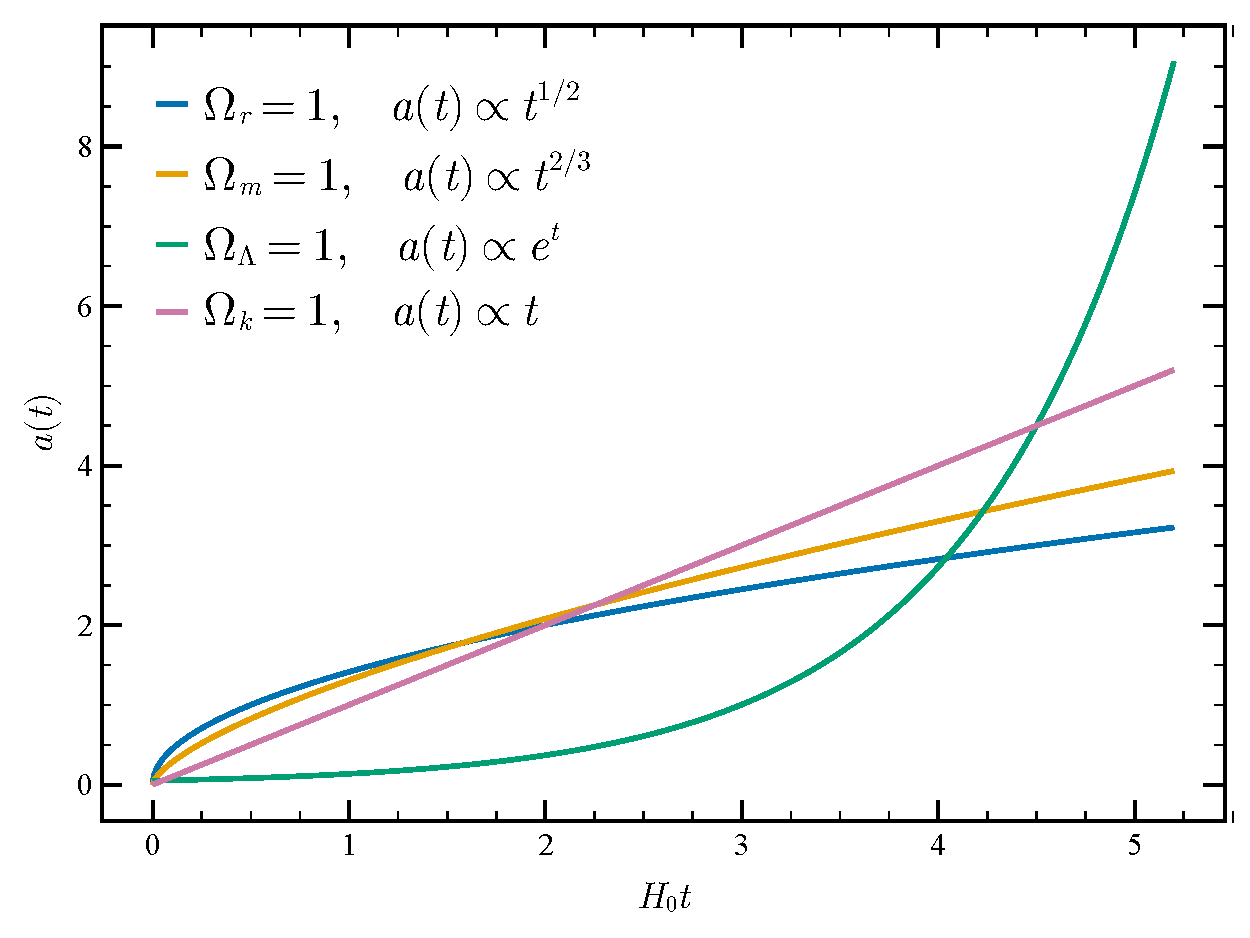
\includegraphics[width=0.85\textwidth]{testplot}
		\end{minipage}
	\tcbline
		\item \(  \)
		\begin{minipage}{\textwidth}
			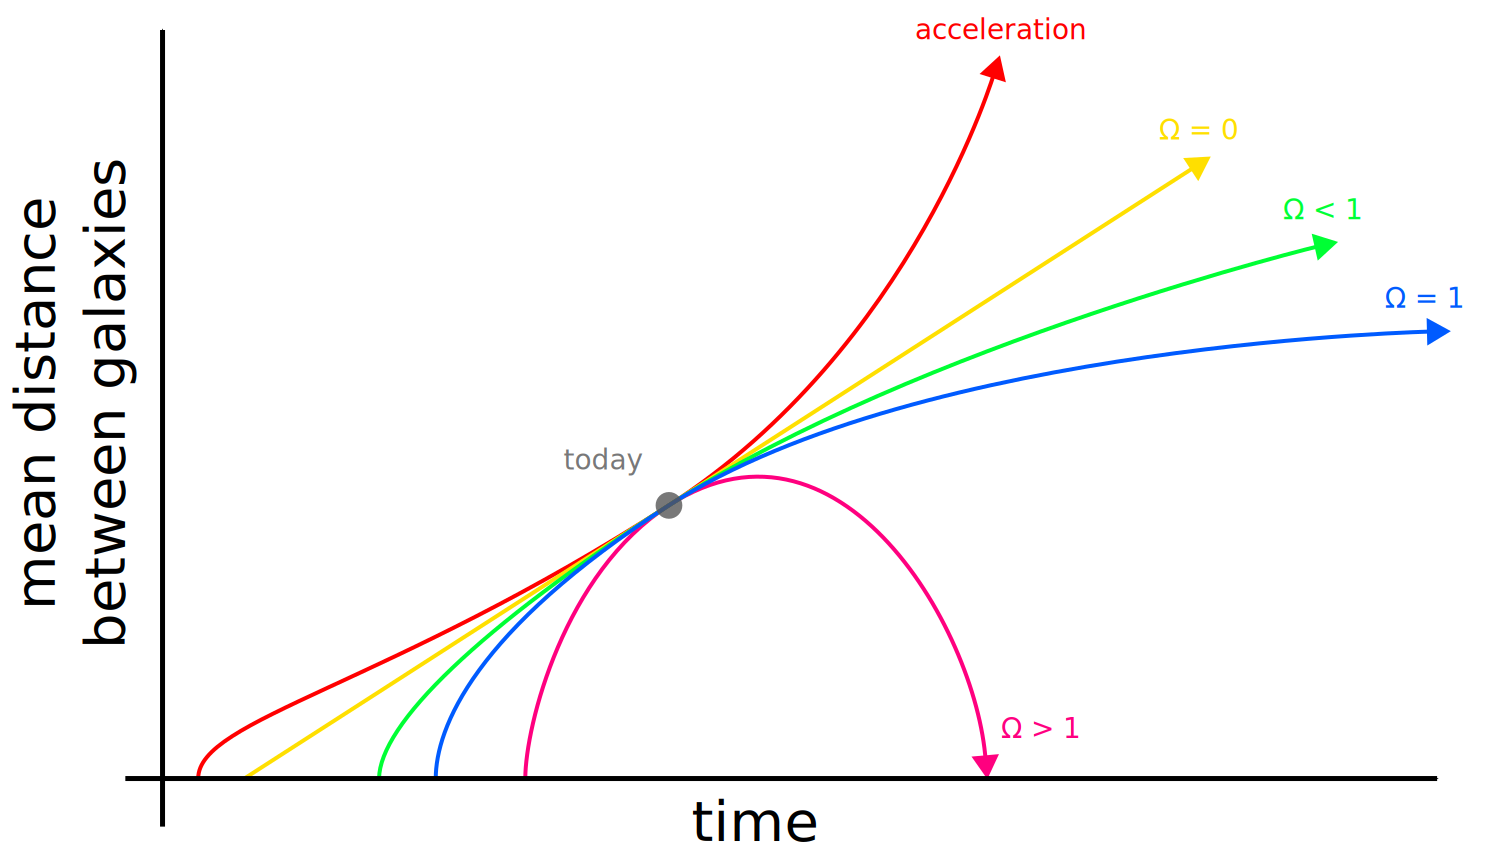
\includegraphics[width=0.85\textwidth]{evo}
		\end{minipage}\vspace{1cm}
		
		\( \Omega_0 < 1 \) leads to a negative Curvature and to an ever expanding Universe \\[1ex]
		\( \Omega_0 = 1 \) leads to zero Curvature and to an expansion, where the rate of expansion approaches zero asymptotically \\[1ex]
		\( \Omega_0 > 1 \) leads to a positive Curvature and to a collapsing Universe \\
	\end{enumerate}
\end{mybox}

\end{document}